\documentclass[a4paper,12pt]{article}
\usepackage[utf8]{inputenc}
\usepackage[russian]{babel}
\usepackage{amsmath}
\usepackage{graphicx}
\usepackage{geometry}
\usepackage{color}
\usepackage{caption}
\usepackage{fancyhdr}
\usepackage{titlesec}
\usepackage{setspace}
\usepackage{float}
\usepackage{booktabs}
\usepackage{multirow}

\geometry{top=2cm,bottom=2cm,left=2cm,right=2cm}

% Настройка заголовков
\titleformat{\section}{\large\bfseries\color{blue}}{}{0em}{}[\titlerule]
\titleformat{\subsection}{\bfseries\color{blue}}{}{0em}{}

% Настройка шапки и подвала
\pagestyle{fancy}
\fancyhf{}
\fancyhead[L]{Классификация распределения с помощью случайных графов}
\fancyhead[R]{\thepage}
\fancyfoot[C]{\textit{Соколовский С.П., Григоренко М.Д.}}

% Настройка интервала между строками
\onehalfspacing

\title{\textbf{Классификация распределения с помощью случайных графов}} 
\author{Соколовский С.П., Григоренко М.Д.}
\date{Дата: \today}

\begin{document}

\maketitle

\section{Предисловие}
Договоримся об обозначениях: \begin{itemize}
    \item $n$ --- размер вектора реализаций случайной величины
    \item $k$, $d$ --- параметры построения KNN и дистанционного графов соответственно
    \item $\theta, v$ --- параметры распределений
    \item $T^{KNN}$, $T^{dist}$ --- характеристики случайных графов
\end{itemize}

\section{Часть I. Исследование свойств характеристики}
\subsubsection*{Используемые инструменты Соколовского С.П.}
Весь код в ветке \texttt{Crazy-Explorer31/first\_part}, в директории \texttt{src/}:
\begin{itemize}
    \item \texttt{graphs.py} --- реализации KNN и дистанционного графов (построение и отрисовка)
    \item \texttt{characteristics\_experimental.py} --- функции для получения характеристик графов, построенных при данных параметрах (распределений, построения графов...). Самая важная --- \texttt{get\_average\_characteristics}, возвращающая средние характеристики графов, построенных при переданных параметрах
    \item \texttt{characteristics\_applied.py} --- функции, возвращающие хар-ки данного графа
    \item \texttt{visualisations.py} --- функции для удобного построения графиков
    \item \texttt{metrics.py} --- функции, приближенно считающие ошибку I рода и мощность для данного $\mathcal{A}$. Считается по методу Монте-Карло, используя переданное в функцию множество точек (число компонент, хроматическое число), принадлежащих какому-то распределению.
    \item \texttt{classifier.py} --- класс, генерирующий характеристики графов по данным параметрам и строящий $\mathcal{A}$ как \textit{жадный рюкзак}
\end{itemize}

\subsubsection*{Используемые инструменты Григоренко М.Д.}
Весь код в ветке \texttt{maxGrigorenko/first\_part}, в директории \texttt{src/}:
\begin{itemize}
    \item \texttt{graph\_common\_functions.py} --- реализации KNN и дистанционного графов (у каждого есть метод для построения из значений случайной величины, а также методы вычисления характеристик)
    \item \texttt{distribution\_functions.py} --- функции для генерации выборки и вычисления матожидания характеристики методом Монте-Карло.
\end{itemize}


\subsection{Шаг 1. Фиксируем $n$. Исследуем взаимосвязь между $\theta, v$ и $T^{KNN}$, $T^{dist}$}
\subsubsection*{Результаты Соколовского С.П.}
В файле \texttt{experiments\_first\_part\_1.ipynb} происходит следующее:
\begin{itemize}
    \item Для каждой тройки (распределение, тип графа, характеристика) перебираются параметры трех перечисленных объектов, после чего вычисляются характеристики полученных графов.
    \item Для каждой тройки строится диаграмма рассеивания, в которой по горизонтальной оси --- параметр распределения, а по вертикальной --- характеристика графа
\end{itemize}
Из графиков заметно, что лишь с дистанционным графом хочется продолжать работать
\subsubsection*{Результаты Григоренко М.Д.}
В файле \texttt{experiments\_first\_part\_1.ipynb} происходит следующее:
\begin{itemize}
    \item Реализованы функции \texttt{plot\_sigma} и \texttt{plot\_beta}, перебирающие значения соответствующих параметров распределений и выводящих график зависимости характеристики графов (knn и dist) от перебираемого параметра
    \item При фиксированном размере выборки проведены эксперименты с различными параметрами $d$ и $k$.
\end{itemize}
В результате всех экпериментов delta графа knn была константной, то есть
эта характеристика никак не связана с параметрами распределений. А вот доминирующее число дистанционного графа в среднем увеличивалось при увеличении параметра sigma. На двух графиках ниже показана зависимость среднего числа характеристик в завимости от параметров распределений: \newline
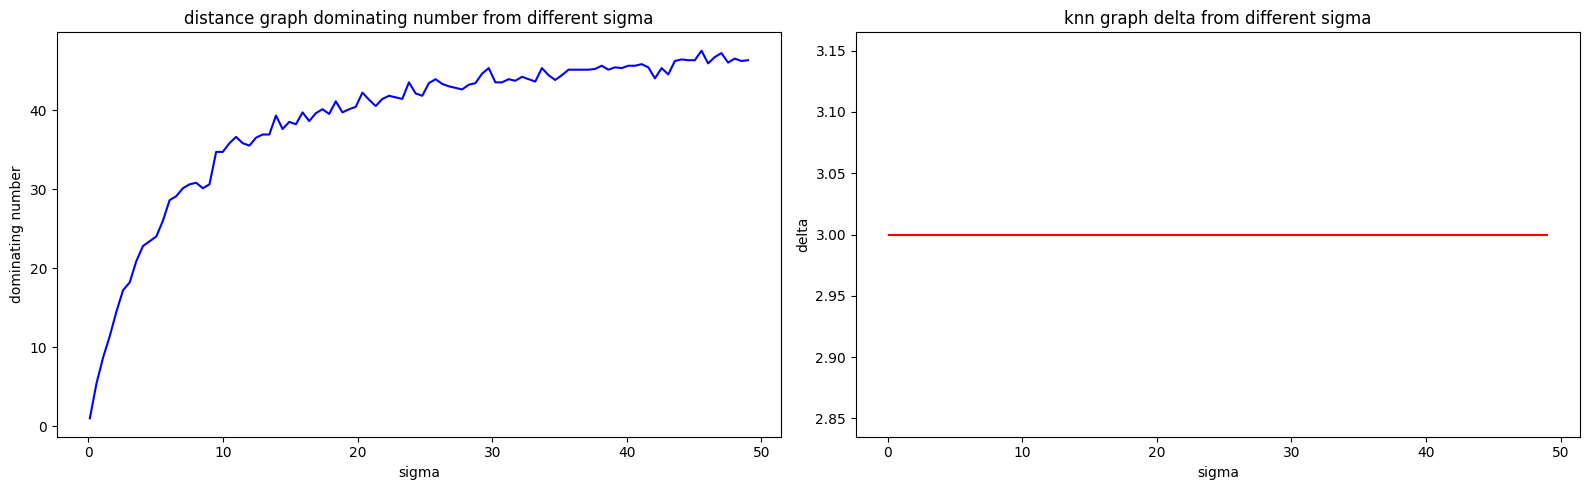
\includegraphics[width=\textwidth]{images/sigma_plot.png}  \newline
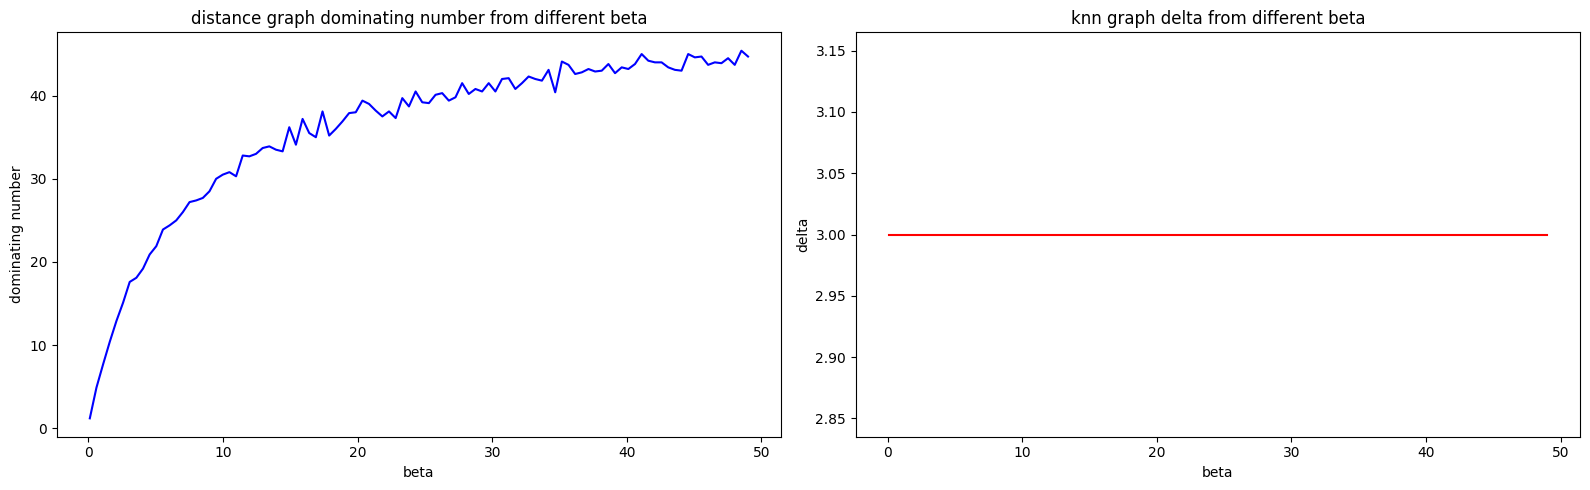
\includegraphics[width=\textwidth]{images/beta_plot.png} \newline

\subsection{Шаг 2. Фиксируем $\theta, v$. Исследуем взаимосвязь между $n$, $k$, $d$ и $T^{KNN}$, $T^{dist}$}
\subsubsection*{Результаты Соколовского С.П.}
В файле \texttt{experiments\_first\_part\_2.ipynb}, аналогично первому шагу, генерятся много налюдений для всех комбинаций распределений, типов графов, их характеристик. Далее на диаграммах рассеивания по оси Ox откладываются параметры построения графов, по Oy --- их характеристики, и ещё цветом отражена, при каком $n$ было получено наюлюдение. Выводы аналогичные первому эксперименту
\subsubsection*{Результаты Григоренко М.Д.}
В файле \texttt{experiments\_first\_part\_2.ipynb} зафиксированы параметры распределений и отрисованы графики зависимости характеристик графов от размера выборки. delta графа knn оказалась неинформативной характеристикой. А вот доминирующее число дистанционного графа немного по-разному меняется при изменении размера выборки, в особенности, если в качестве параметра дистанционного графа установить значение $d >= 3$, то характеристика графа из нормального распределения становится почти всегда равной 1, а вот при распределении Лапласа немного больше. Снизу график зависимости среднего числа доминирования от размера выборки при $d = 3.5$: \newline
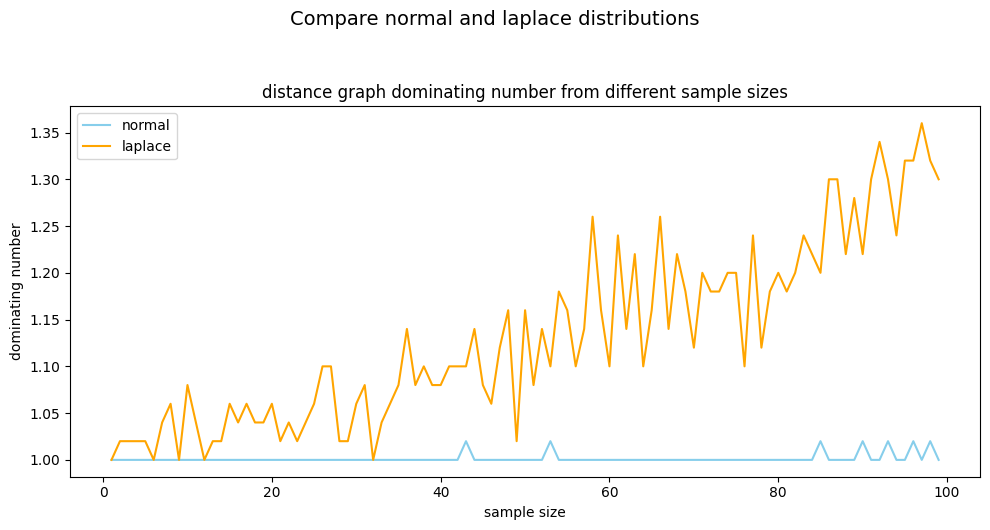
\includegraphics[width=\textwidth]{images/dominating_number_plot.png}

\subsection{Шаг 3. Фиксируем $\theta, v$. Строим $\mathcal{A}$ для переданного $n$}
\subsubsection*{Результаты Соколовского С.П.}
Файл \texttt{experiments\_first\_part\_3.ipynb} поделен на два раздела. В первом фиксируются все параметры и строится $\mathcal{A}$. Во втором рассуждения, изложенные в первом разделе обобщаются, и приведена реализация класса, строящая $\mathcal{A}$ по переданному в конструктор $n$ \\
Используется следующий алгоритм построения $\mathcal{A}$:
\begin{itemize}
    \item[1.] Строятся точки с координатами (число компонент, хроматическое число) по генерирующимся векторам случайных величин
    \item[2.] За изначальное $\mathcal{A}$ берется множество всех сгенерированных точек, полученных по первому распределению (Exp).
    \item[3.] Далее пытаемся удалить точку из $\mathcal{A}$ так, чтобы ошибка I рода не превысила 0.05, а мощность была максимальной (ошибка I рода и мощность считаются на основе точек, сгенерированных в начале). Для этого перебираем все варианты и выбираем наилучший
    \item[4.] Пытаемся так удалить что-то из $\mathcal{A}$ много раз
    \item[5.] В итоге получаем искомое $\mathcal{A}$
\end{itemize}
\subsubsection*{Результаты Григоренко М.Д.}
В файле \texttt{experiments\_first\_part\_3.ipynb} реализован алгоритм конструирования множества $\mathcal{A}$, которое должно удовлетворять двум условиям:

\begin{itemize}
\item[1.] Контроль ошибки первого рода: вероятность ошибочно отвергнуть нулевую гипотезу $H_0$ (данные имеют нормальное распределение) при её справедливости не превышает $\alpha = 0.05$.

\item[2.] Максимизация мощности: вероятность корректно отвергнуть $H_0$ в пользу альтернативы $H_1$ (например, распределение Лапласа) должна быть максимальной.
\end{itemize}

Множество $\mathcal{A}$ конструируется итеративно следующим образом:
На каждом шаге генерируется большое число выборок (number\_of\_experiments) из нормального распределения. Для каждой выборки вычисляется характеристика графа. Если значение характеристики не принадлежит текущему множеству $\mathcal{A}$, оно считается "ошибочным" (ложным отклонением $H_0$). Ошибка первого рода оценивается как доля таких "ошибочных" случаев:
Пока ошибка $\text{err} > \alpha$, в $\mathcal{A}$ добавляется наиболее частое значение характеристики из "ошибочных" результатов (мода). Это снижает долю ошибок за счёт включения типичных для $H_0$ значений.
Процесс останавливается, когда $\text{err} \leq \alpha$, либо когда "ошибочные" значения исчерпаны.

\section{Часть II. Несколько характеристик проверки гипотезы}
\subsection{Шаг 1. Исследуем важность характиристик}
\subsubsection*{Результаты Соколовского С.П.}
В файле \texttt{experiments\_second\_part\_1.ipynb} исследование важности характеристик состоит из визуальной и аналитической частей. В визуальной с помощью функции \\ \texttt{describe\_features\_importances} для разных $n$ построены матрицы скатерплотов, изображающих взаиморасположение точек с координатами, равными характеристикам графов, соответствующим векторам чисел из экспоненциального и Парето распределений. Заметно, что при росте $n$ граница между точками разного характера становится очевиднее. 
\hspace{-10cm} 
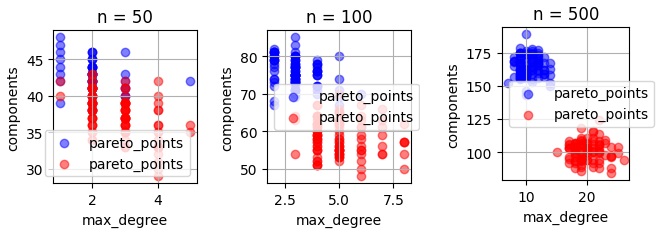
\includegraphics[width=\textwidth]{images/plots.png}
\hspace{+10cm} 
В аналитической части важность признаков изучается с помощью случайного леса: для разных $n$ на сгенерированных данных обучается случайный лес (с перебором гиперпараметров), а затем с помощью встроенного метода класса случайного леса из sklearn достаются важности признаков. Ниже представлена гистограма важностей признаков для $n = 500$.
\hspace{-5cm} 
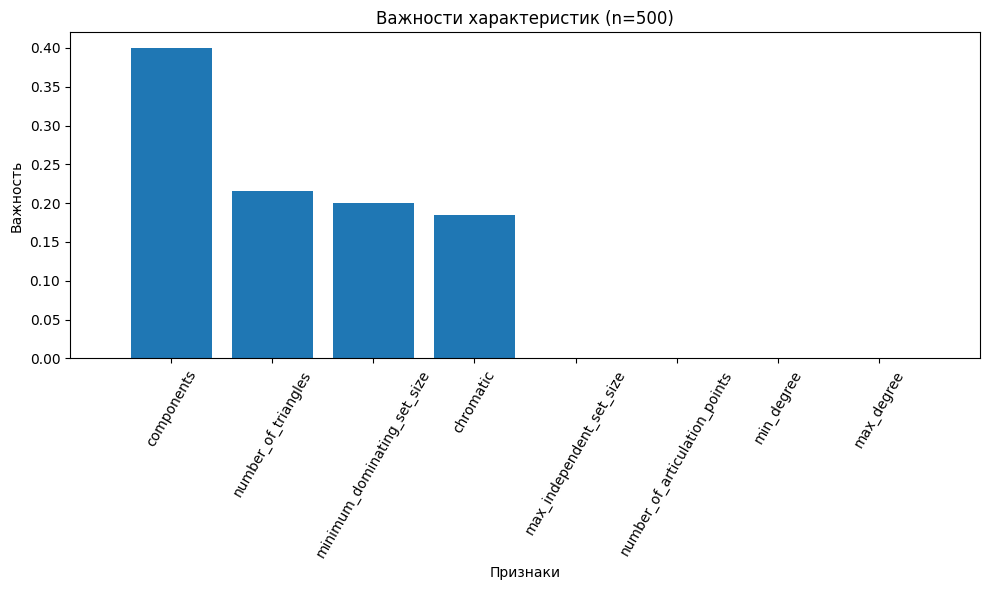
\includegraphics[width=\textwidth]{images/imps.png}
\hspace{+5cm}
При обучении моделей буду использовать именно эти четыре характеристики: число компонент, число треугольников, размер наименьшего доминирующего множества, хроматическое число.
\subsubsection*{Результаты Григоренко М.Д.}
В файле \texttt{experiments\_second\_part.ipynb} написан класс \texttt{DistribituionClassifier}, принимающий на вход параметр $n$ - размер выборки и модель классификации, которую предстоит обучить. Для выявление признаков по данной выборке строится 4 дистанционных графа с различным параметром $d$, для каждого графа считаеются следующие характеристики:
\begin{itemize}
    \item[1.] Минимальная степень вершины
    \item[2.] Средняя степень вершины
    \item[3.] Максимальная степень вершины
    \item[4.] Число доминирования
    \item[5.] Кликовое число
\end{itemize}
Важность характеристик слабо меняется при разных n. Самыми важными характеристиками оказались средняя и максимальная степени дистанционного графа при $d = 0.3$ (самое маленькое значени $d$). Ниже предствлена гистограмма важности признаков при $n = 500$: \newline
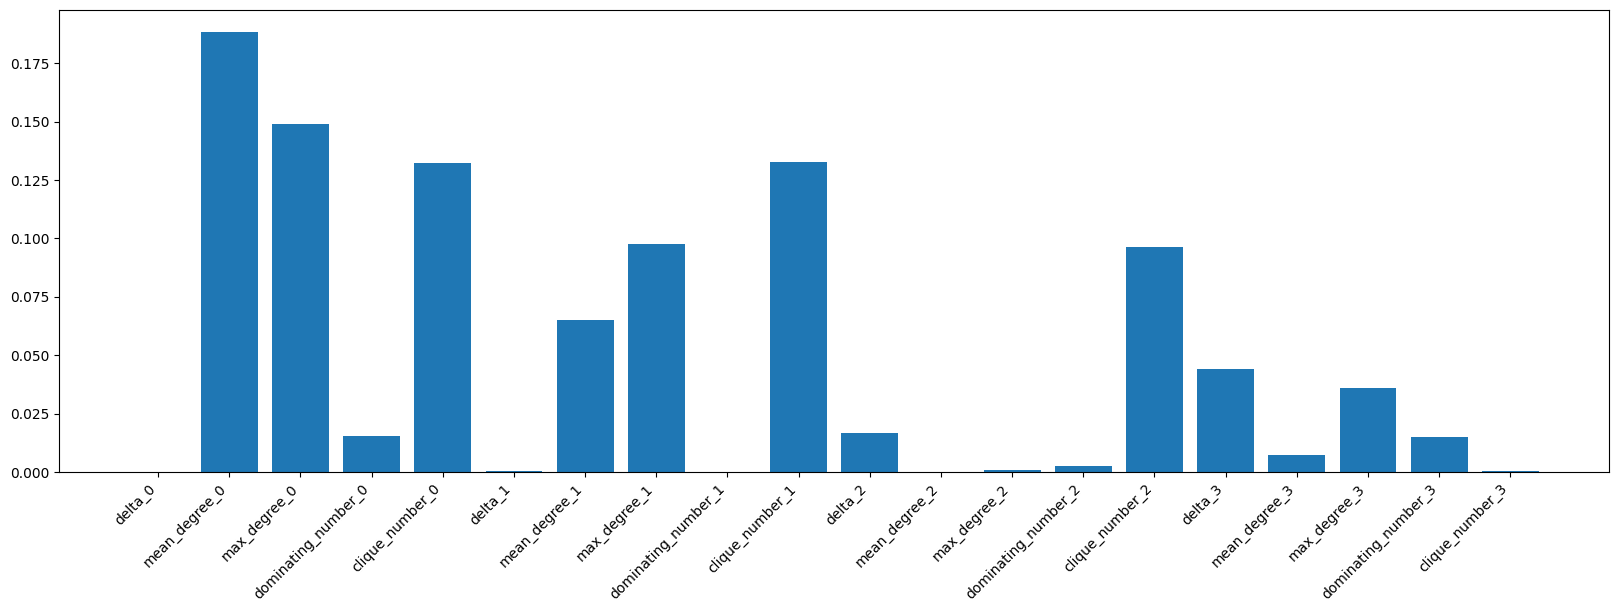
\includegraphics[width=\textwidth]{images/importances_barplot.png}


\subsection{Шаг 2. Обучаем разные модели и мерим качество для разных размеров $\hat{\xi}$}
\subsubsection*{Результаты Соколовского С.П.}
Всё в файле \texttt{experiments\_second\_part\_2.ipynb}.
Для данной задачи были опробованы следующие модели: жадная (формирующая $\mathcal{A}$ как в задаче про рюкзак), случайный лес, логистическая регресия. Пройдемся по каждой:
\begin{itemize}
    \item[1.] Реализация в \texttt{classifier.py}. Жадник работал следующим образом: сперва генерировались характеристики (далее --- точки с их координатами) для графов разных распределений, затем $\mathcal{A}$ инициализировалось как множество уникальных точек экспоненциального распределения, и, наконец, в цикле, пока ошибка I рода не превышает 0.05, из $\mathcal{A}$ выкидывалась точка так, чтобы максимально увеличить мощность. Отмечу, что здесь за $\mathcal{A}$ берется не множество точек, а их выпуклая оболочка (статистический критерий --- принадлежность данной точки этой выпуклой оболочке). Из-за вычислительной сложности, качественно удалось обучить лишь для $n = 75$
    \begin{center}
    \hspace{-2cm} % или другое значение
    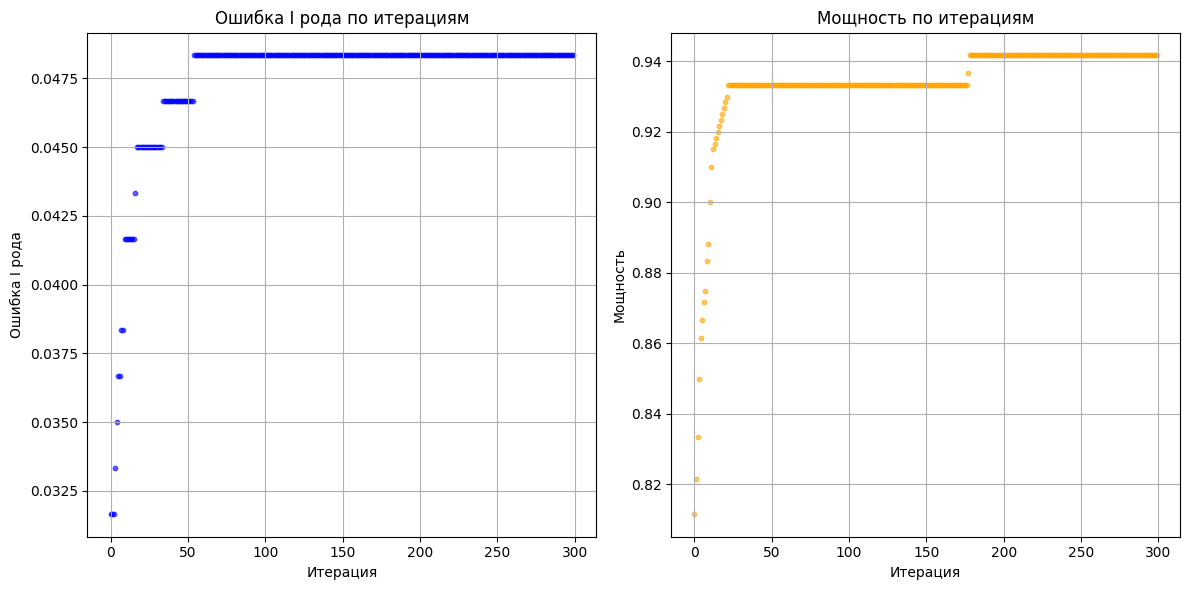
\includegraphics[width=\textwidth]{images/erros_powers.png}
    \hspace{+2cm} % или другое значение
    \end{center}
% \newpage
    \begin{table}
    \centering
    \begin{tabular}{|c|c|c|c|c|c|c|c|}
        \hline
        n & Accuracy & Precision & Recall & F1 Score & ROC AUC & I\_error & Power \\
        \hline
        75 & 0.9375 & 0.9397 & 0.935 & 0.9373 & 0.9375 & 0.0483 & 0.9417 \\
        \hline
    \end{tabular}
    \caption*{Метрики модели рюкзака}
    \label{tab:my_label}
\end{table}
\newpage
    \item[2.] По аналогии с предыдущим шагом был обучен случайный лес. Метрики у него тем более выдающиеся, чем больше $n$. Однако, как в предыдущем шаге, контролировать ошибку I рода нельзя (но при больших $n$ необходимость в этом отпадает) \\
    \begin{table}[H]
        \centering
        \begin{tabular}{|c|c|c|c|c|c|c|c|}
            \hline
            n & Accuracy & Precision & Recall & F1 Score & ROC AUC & I\_error & Power \\
            \hline
            50 & 0.8750 & 0.8866 & 0.8600 & 0.8731 & 0.8750 & 0.1100 & 0.8600 \\
            100 & 0.9850 & 0.9802 & 0.9900 & 0.9851 & 0.9850 & 0.0200 & 0.9900 \\
            500 & 1.0000 & 1.0000 & 1.0000 & 1.0000 & 1.0000 & 0.0000 & 1.0000 \\
            \hline
        \end{tabular}
        \caption*{Метрики модели случайного леса}
        \label{tab:random_forest_metrics}
    \end{table}
    \item[3.] Почти такого же качества получилась модель логистической регрессии. Однако преимущество её над случайным лесом в том, что, варьируя её пороговое значение, мы можем контролировать ошибку I рода (пока не актуально --- работает хорошо из коробки)
    \begin{table}[H]
    \centering
    \begin{tabular}{|c|c|c|c|c|c|c|c|}
        \hline
        n & Accuracy & Precision & Recall & F1 Score & ROC AUC & I\_error & Power \\
        \hline
        50 & 0.8575 & 0.8865 & 0.8200 & 0.8519 & 0.8575 & 0.1050 & 0.8200 \\
        100 & 0.9850 & 0.9899 & 0.9800 & 0.9849 & 0.9850 & 0.0100 & 0.9800 \\
        500 & 1.0000 & 1.0000 & 1.0000 & 1.0000 & 1.0000 & 0.0000 & 1.0000 \\
        \hline
    \end{tabular}
    \caption*{Метрики модели логистической регрессии}
    \label{tab:logistic_regression_metrics}
\end{table}
\end{itemize}

\subsubsection*{Результаты Григоренко М.Д.}
Для каждого $n$ (размер выборки) были обучены классификаторы \texttt{RandomForestClassifier}, с подобранными гиперпараметрами \texttt{max\_depth} и \texttt{min\_samples\_split}, и \texttt{BaggingClassifier} c подобранным гиперпараметром \texttt{n\_estimators} (из библиотеки \texttt{sklearn}). Для всех выборок чуть лучше (или примерно одинаково) оказался классификатор \texttt{RandomForestClassifier}. Лучшие метрики (за положительный класс взято $H_1$ (распределение Лапласа)):
\begin{itemize}
    \item[1.] $n = 25$: \texttt{accuracy = 0.77, precision = 0.79, recall = 0.74.}. Измерение проводилось на 2000 примерах.
    \item[2.] $n = 100$: \texttt{accuracy = 0.95, precision = 0.94, recall = 0.96}. Измерение проводилось на 200 примерах.
    \item[3.] $n = 500$: \texttt{accuracy = 1.0, precision = 1.0, recall = 1.0}. Измерение проводилось на 200 примерах (из-за сложности построения дистанционного графа на 500 вершинах).
\end{itemize}

\subsection{Шаг 3. Выводы о вероятности ошибки первого рода и мощности подхода}
\subsubsection*{Результаты Соколовского С.П.}
В качестве исследуемой архитектуры взята логистическая регрессия (потому что она лучше рюкзака и всё ещё можно контролировать ошибку I рода). Измерение метрик проводилось так: для каждого $n \in \{50, 100, 500 \}$ обучалась модель выбранной архитектуры, 10 раз измерялись её метрики на новых сгенерированных точках, а затем брались статистики по полученным метрикам. При $n = 50$, для модели пришлось взять threshold равным 0.8, чтоб ошибка I рода была небольшая. Ниже приведены результаты этих измерений
\begin{table}[H]
    \centering
    \begin{tabular}{ccc}
        \begin{tabular}{|c|c|c|}
            \hline
            \multicolumn{3}{|c|}{n = 50} \\
            \hline
            & I\_error & Power \\
            \hline
            min  & 0.019868 & 0.6150 \\
            \hline
            mean & 0.041746 & 0.6705 \\
            \hline
            max  & 0.058824 & 0.7400 \\
            \hline
        \end{tabular} &

        \begin{tabular}{|c|c|c|}
            \hline
            \multicolumn{3}{|c|}{n = 100} \\
            \hline
            & I\_error & Power \\
            \hline
            min  & 0.000000 & 0.945 \\
            \hline
            mean & 0.014645 & 0.969 \\
            \hline
            max  & 0.029557 & 0.985 \\
            \hline
        \end{tabular} &

        \begin{tabular}{|c|c|c|}
            \hline
            \multicolumn{3}{|c|}{n = 500} \\
            \hline
            & I\_error & Power \\
            \hline
            min  & 0.0 & 1.0 \\
            \hline
            mean & 0.0 & 1.0 \\
            \hline
            max  & 0.0 & 1.0 \\
            \hline
        \end{tabular} \\
    \end{tabular}
    \caption*{Статистики по метрикам логистической регрессии по разным $n$}
    \label{tab:three_tables}
\end{table}

\subsubsection*{Результаты Григоренко М.Д.}
Мощность критерия по определению равна метрике \texttt{recall}. Вероятность ошибки первого рода была измерена отдельно:
\begin{itemize}
    \item[1.] $n = 25$: \texttt{error = 0.22}. Измерение проводилось на 2000 примерах.
    \item[2.] $n = 100$: \texttt{error = 0.055}. Измерение проводилось на 2000 примерах.
    \item[3.] $n = 500$: \texttt{error = 0.0}. Измерение проводилось на 200 примерах (из-за сложности построения дистанционного графа на 500 вершинах). Таким образом, можно оценить ошибку сверху \texttt{error < 0.01}.
\end{itemize}
\section{Заключение}
В ходе работы были успешно подобраны модели для классификации распределения случайной величины по данному вектору из её реализаций:
\begin{itemize}
    \item Для классификации \textit{Нормальное} $\leftrightarrow$ \textit{Лаплас} --- \texttt{RandomForest}
    \item Для классификации \textit{Экспоненциальное} $\leftrightarrow$ \textit{Парето} --- \texttt{LogisticRegression}
\end{itemize}
Также было замечено, что при увеличении $n$ качество модели повышается, так как характеристики графов разной природы становятся более "непохожими". \\
Данная работа свидетельствует о том, что такие абстрактные объекты, как случайные графы, имеют хорошее практическое применение. В данном случае --- при проверке гипотезы согласия

\end{document}
